% --------------------------------------------------------------
% This is all preamble stuff that you don't have to worry about.
% Head down to where it says "Start here"
% --------------------------------------------------------------

\documentclass[12pt]{article}

\usepackage[margin=1in]{geometry}
\usepackage{amsmath,amsthm,amssymb}
\usepackage{graphicx}
\usepackage{subcaption}
\usepackage{algorithmicx}
\usepackage{algorithm}
\usepackage{algpseudocode}
\usepackage[colorlinks,linkcolor=blue]{hyperref}
\usepackage[noabbrev]{cleveref}
\usepackage{courier}
\usepackage{listings}

\oddsidemargin 0in
\evensidemargin 0in
\textwidth 6.5in
\topmargin -0.5in
\textheight 9.0in
\graphicspath{{./images}}

\newcommand{\ignore}[1]{}
\def\pp{\par\noindent}

\newcommand{\assignment}[4]{
\thispagestyle{plain}
\newpage
\setcounter{page}{1}
\noindent
\begin{center}
\framebox{ \vbox{ \hbox to 6.28in
{CIS 419/519: Applied Machine Learning \hfill #1}
\vspace{4mm}
\hbox to 6.28in
{\hspace{2.5in}\large\bf\mbox{Homework #2}}
\vspace{4mm}
\hbox to 6.28in
{{\it Handed Out: #3 \hfill Due: #4}}
}}
\end{center}
}

\makeatletter
\renewcommand{\fnum@algorithm}{\fname@algorithm}
\makeatother

\lstset{basicstyle=\footnotesize\ttfamily,breaklines=true}
\lstset{framextopmargin=50pt,frame=bottomline}


\begin{document}

\assignment{Fall 2024}{2}{October 2}{7:59 pm October 22}

% --------------------------------------------------------------
%                         Start here
% --------------------------------------------------------------


{\bf Name: }  Yueyang Li\\

{\bf PennKey:} ezel22\\

{\bf PennID:} 47700221\\

{\bf E-mail:} ezel22@seas.upenn.edu


\section{Declaration}
\begin{itemize}
\item \textbf{Person(s) discussed with:} \textit{None}
\item \textbf{Affiliation to the course: student, TA, prof etc.} \textit{None}
\item \textbf{Which question(s) in coding / written HW did you discuss?} \textbf{\textit{None}}
\item \textbf{Briefly explain what was discussed.} \textit{None}
\end{itemize}

\section{Multiple Choice \& Written Questions}

\begin{enumerate}
\item 
\begin{enumerate}
\item Bias: Stays roughly the same ; Variance:increases
\item Bias: increases ; Variance:decreases 
\item Bias: increases ; Variance decrease 
\item bias remains roughly the same, variance remains the same
\item bias remains roughly the same, variance remains roughly the same
\item 
The strategy that we will apply is below: \\
- increase the n, as more samples will significantly decrease the variance, and keep the bais roughly the same, making the model less likely to overfit the training data and performs better in test dataset(reduce the test loss) \\
- increase the \( lambda \) since it will apply stronger regularization on the training, and will significantly reduce the chance of overfitting the training dataset and thus reduce the test loss \\
- Decrease the \( d \), since lowering the number of features will decrease the chance of overfitting the training dataset (simpler model), thus it will perform better, in reducing the test loss in test dataset. \\
- whether \(\mathbf{increasing}\) or decreasing \( c \) has no impact.
\end{enumerate}

\item
\begin{enumerate}
\item The gradient of regularization term of a single weight is:\\
\[
\frac{d}{d\beta} \lambda|\beta_j| = \lambda \text{ if } \beta_j > 0 \text{ or } -\lambda \text{ if } \beta_j < 0
\]
Hence, we can say that:
\[
\frac{\partial}{\partial \beta_j} \lambda|\beta_j| = \lambda \cdot \textbf{sign}(\beta_j)
\]
\item We can explain the effect in the following reasoning:\\
When taking a look at the partial differential derivative with respect to $\beta_j$ being one scalar weights of $\beta$:
\[
\frac{\partial}{\partial \beta_j}\L_{loss} = -2 \cdot \frac{1}{N} \sum_{i = 1}^{N} x_{i,j}(y_i - \beta^T x_i) + \lambda \textbf{sign}(\beta_j)
\]
By investigating into this partial differential derivatives, we can see that, the gradient(actually partial differnetial) with respect to \(\beta_j\) (partial differentiation):
the term: \(-2 \frac{1}{N} \sum_{i = 1}^{N} x_{i,j} (y_i - \beta^{T} x_i)\) becomes very small or negligible when $\beta_j$ is close to \(0\).  \\
On the other hand, $\lambda \textbf{sign}(\beta_j)$ provides a negative contribution to where the $beta_j$ is contributing to the derivative, pushing the final results towards \(0\).
Therefore, based on the above effect, it explains why when \(\beta_j\)  is closed to \(0\), the gradient contributed by \(\beta_j\) also tends to be \(0\) and thus have the effect of feature selection.

\item For \(L_2\) regularization, the gradient of the regularization term with respect to \(\beta_j\) is:
\[
\frac{\partial}{\partial \beta_j} \lambda \beta_{j}^{2} = 2 \lambda \beta_{j}
\]
Unlike \(l_1\) regularization, this term is proportional to \(\beta_j\) itself, it continuously shrinks \(\beta_j\), thus, even when \(\beta_j\) is extremely close to \(0\), it doesn't actually gets to \(0\). Therefore, the conclusion is, \(l_2\) regularization doesn't create sparsity. It reduces the magnitude of the weights but doesn't perform feature selection in the same way as \(l_1\) regularization does.
\end{enumerate}

\item
  \begin{enumerate}
  \item The derivatives $w_{0}^{*}, w_{1}^{*}$ is found by:
  Derivative with respect to $w_0$ :

$$
\frac{\partial}{\partial w_0} J(\mathbf{w})=\frac{1}{n} \sum_{i=1}^n 2\left(y_i-w_0-w_1 x_i\right)(-1)
$$


Simplifying:

$$
\frac{\partial}{\partial w_0} J(\mathbf{w})=-\frac{2}{n} \sum_{i=1}^n\left(y_i-w_0-w_1 x_i\right)
$$


Derivative with respect to $w_1$ :

$$
\frac{\partial}{\partial w_1} J(\mathbf{w})=\frac{1}{n} \sum_{i=1}^n 2\left(y_i-w_0-w_1 x_i\right)\left(-x_i\right)
$$


Simplifying:

$$
\frac{\partial}{\partial w_1} J(\mathbf{w})=-\frac{2}{n} \sum_{i=1}^n\left(y_i-w_0-w_1 x_i\right) x_i
$$

  \item we can show the proof by the folloiwng statement:\\
  
$$
\frac{1}{n} \sum_{i=1}^n\left(y_i-w_0^*-w_1^* x_i\right)\left(x_i-\bar{x}\right)=0
$$


First, recall that $w_0^*$ and $w_1^*$ represent the optimal values for the weights that minimize the cost function $J(\mathbf{w})$.

Start with the gradient equation with respect to $w_1$, which we found to be:

$$
\frac{\partial}{\partial w_1} J(\mathbf{w})=-\frac{2}{n} \sum_{i=1}^n\left(y_i-w_0^*-w_1^* x_i\right) x_i=0
$$


Multiplying through by $\frac{n}{2}$ :

$$
\sum_{i=1}^n\left(y_i-w_0^*-w_1^* x_i\right) x_i=0
$$


Now, rewrite the term on the left-hand side:

$$
\sum_{i=1}^n\left(y_i-w_0^*-w_1^* x_i\right)\left(x_i-\bar{x}+\bar{x}\right)
$$


Expanding this:

$$
\sum_{i=1}^n\left(y_i-w_0^*-w_1^* x_i\right)\left(x_i-\bar{x}\right)+\sum_{i=1}^n\left(y_i-w_0^*-w_1^* x_i\right) \bar{x}
$$


The second sum simplifies to zero because the term $\left(y_i-w_0^*-w_1^* x_i\right)$ is constant and its sum wit $\bar{x}$ gives zero due to the optimality condition (it equals zero for optimal weights).
    \item I believe the answer is no.\\
    Multicollineartiy: if multiple features are colinear, then there might not be unique solution.
    
  \end{enumerate}

\item
  \begin{enumerate}
  \item first, let's organize the information we have so far:\\
    \(x_n \in \mathbb{r}^2 \textbf{ and } y_n \in \{ 0, 1\}\) \\
    batch gradient descent is applied\\
    thus
    \[
    l=\frac{1}{n} \sigma_{i=1}^n\left(y_i-w x_i\right)^2+\lambda\|w\|^2
    \]
    plug in the value that \(w = 0\), we can obtain the loss function value:
    \[
    l_{val} = 0.5
    \]
    
  \item 
  we can obtain the partial derivative of the loss function be:
  \[
  \frac{\partial}{\partial \omega_j}\l_{2} = -2 \cdot \frac{1}{2} \sum_{i = 1}^{n} x_{i,j}(y_i - \omega^t x_i) + 2 \lambda \omega_{j}
  \]
  where \(x_{i,j}\) represents the \(i\)th and \(j\)th element in the x matrix of \(n \times d\). \
  by plugging into the value, the result will be:\\
  initial: [0, 0]\\
  
  1 st round:
  \[
  \frac{\partial}{\partial \omega_1} = -(1(0-0) + (-1)(1-0)) + 2(0) = 1
  \]
  \[
  \frac{\partial}{\partial \omega_2} = -((-1)(0 - 0) + (-1)(1-0)) + 2(0) = 1
  \]
  So after the 1st iteration, the result should be:\\
  \(\vec{\omega} = [-1, -1]^T\) \\
  2nd round: [2, 2]
  \[
  \frac{\partial}{\partial \omega_1} = -(1 \cdot (0-0) + (-1)(1 -2)) + 2(-1) = -3 
  \] 
  \[
  \frac{\partial}{\partial \omega_2} = -((-1)\cdot (0-0) + (-1)(1 -2)) + 2(-1) = -3
  \]
  So after the 2nd iteration, the result should be:\\
  \(\vec{\omega} = [2, 2]^T\) \\
  Compute the Loss:
  Since we obtained the \(\omega_{i}\) after \(2^{nd}\) iteration to be \([2, 2]\):\\
  By plugging this value into the formula of calculating the loss:\\
  \[
  \L = \frac{1}{2} \cdot ((0 - (2 \cdot 1 +  2 \cdot (-1)))^2 + ((1 - (2 \cdot (-1) + 2 \cdot (-1))))^2 + 1 \cdot (2 + 2) = 13 / 2 = 12.5
  \]
  
  
  \item So first  and foremost, we need to vectorize the ridge Regression form
  \[
  L(\mathbf{w})=\frac{1}{N}(\mathbf{y}-\mathbf{X} \mathbf{w})^T(\mathbf{y}-\mathbf{X} \mathbf{w})+\lambda \mathbf{w}^T \mathbf{w}
  \]
  Take the gradient of the loss function, we can get:
  \[
  \nabla_{\mathbf{w}} L(\mathbf{w})=\frac{2}{N} \mathbf{X}^T \mathbf{X} \mathbf{w}-\frac{2}{N} \mathbf{X}^T \mathbf{y}+2 \lambda \mathbf{w}
  \]
  By setting the derivative to \(0\), we can get:
  \[
  \left(\mathbf{X}^T \mathbf{X}+N \lambda \mathbf{I}\right) \mathbf{w}=\mathbf{X}^T \mathbf{y}
  \]
  So we can get the ridge regression closed-form solution as:
  
  \[
  \mathbf{w}=\left(\mathbf{X}^T \mathbf{X}+N \lambda \mathbf{I}\right)^{-1} \mathbf{X}^T \mathbf{y}
  \]

  \end{enumerate}
\end{enumerate}

\section{Python Programming Questions}
    \begin{figure}[h]
    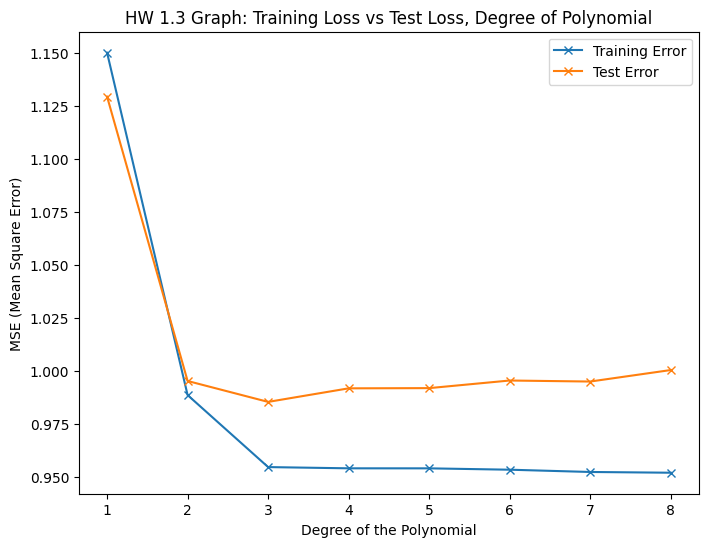
\includegraphics{images/hw01_Graph1.3_PolynomialDegreeLoss.png} 
    \end{figure}
    \begin{figure}[h]
    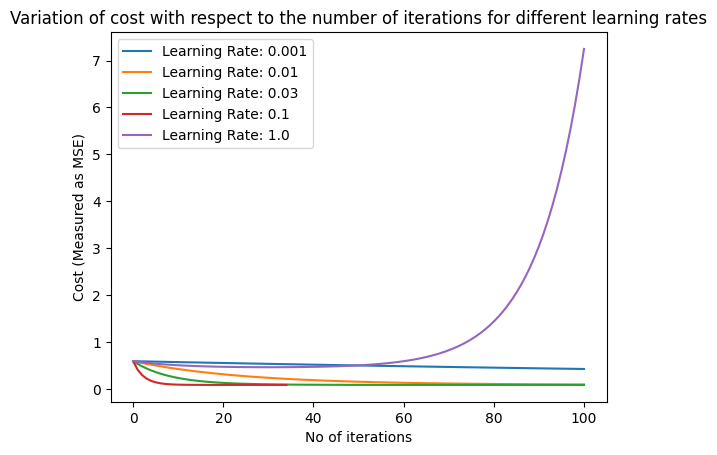
\includegraphics{images/hw01_Graph1.4_Graph_Different_LearningRate.png}
    \end{figure}
% Complete questions in your iPython notebook and place all results here.

\end{document} 